%This is a TeX file which when compiled generates a pdf with all the dossiers from all filters
%This file provides a full report.
%----Begin Preamble----%
\documentclass[11pt,twoside,letterpaper]{article}

\usepackage[margin=2.5cm]{geometry}
\usepackage{fancyhdr}
\usepackage{type1cm} % scalable
\usepackage{lettrine}
\usepackage{graphicx}
\usepackage{booktabs}
\usepackage{multirow}
\usepackage{amsmath}
\usepackage[table]{xcolor}
\usepackage{colortbl}
\usepackage{longtable}
\usepackage[raggedright]{sidecap}
\setlength{\headheight}{14pt}

%----End Preamble----%
%----Begin Document----%
\begin{document}

%Header and footer
\pagestyle{fancy}
\lhead{}
\chead{}
\rhead{\bfseries Summary of results}
\lfoot{http://chiron.dokhlab.org}
\cfoot{\thepage}
\rfoot{\today}
\renewcommand{\headrulewidth}{0.4pt}
\renewcommand{\footrulewidth}{0.4pt}

%Introduction
\lettrine[lines=3,nindent=-1pt]{G}{aia} evaluates the quality of a given protein structure or a structural model based on different criteria. The statistics used by Gaia for comparison are generated from high resolution crystal structures. The observed and expected scores for different criteria used by Gaia to score the given structure are summarized in the table below. Values in cells with a red background indicate parameters that need immediate attention in order to refine the structure further.

\vspace{0.75cm}\noindent\framebox[6.45in]{\parbox[bt]{6.45in}{\centering{This report is generated by Gaia, developed by the Dokholyan group. \\Please cite : Kota, P., Ding, F., Ramachandran, S. and Dokholyan N.V. Bioinformatics (2011)}}}

%Summary table
\begin{table}[!h]
	\textbf{\caption{Summary of scores for the input structure}}
	\begin{center}
		\begin{tabular}{l@{\hspace{1cm}}c@{\hspace{1cm}}cc}
		\toprule%
		\multicolumn{2}{l}{\cellcolor[gray]{0.9} \textbf{Criterion}} & \cellcolor[gray]{0.9} \textbf{Observed} & \cellcolor[gray]{0.9} \textbf{Target} \\\midrule
		\multicolumn{2}{l}{Steric clashes} & \cellcolor{white}0.02 & 0.02\\\midrule
		\multirow{2}{*}{Hydrogen bonds}  & \%Unsatisfied in shell & \cellcolor{white}13.80 & 9.56\\\cmidrule(r){2-4}
			& \%Unsatisfied in core & \cellcolor{white}1.30 & 1.45\\\midrule
		\multicolumn{2}{l}{Solvent accessible surface area} & \cellcolor{white}190.55 & 221.64\\\midrule
		\multicolumn{2}{l}{Void volume} & \cellcolor{purple!50!white}0.50 & 0.097\\\midrule
	\end{tabular}
	\end{center}
\end{table}

%Steric Clashes
\newpage
\begin{table}[!h]
	\begin{center}
		\begin{tabular}{p{16.1cm}}
			\midrule
			\cellcolor[gray]{0.9}\textbf{Steric clashes}\\
			\midrule
		\end{tabular}
	\end{center}
\end{table}
\begin{table}[!h]
	\begin{center}
		\begin{tabular}{l@{\hspace{1cm}}c}
		\toprule
		\multicolumn{2}{c}{\cellcolor[gray]{0.9} \textbf{Clash summary}} \\
			\midrule
			Number of residues & 102\\
			Number of contacts & 1353\\
			Number of clashes & 35\\
			Clash score & 0.02\\
			\midrule
		\end{tabular}
	\end{center}
\end{table}

\begin{figure}[h!]
	\begin{center}
		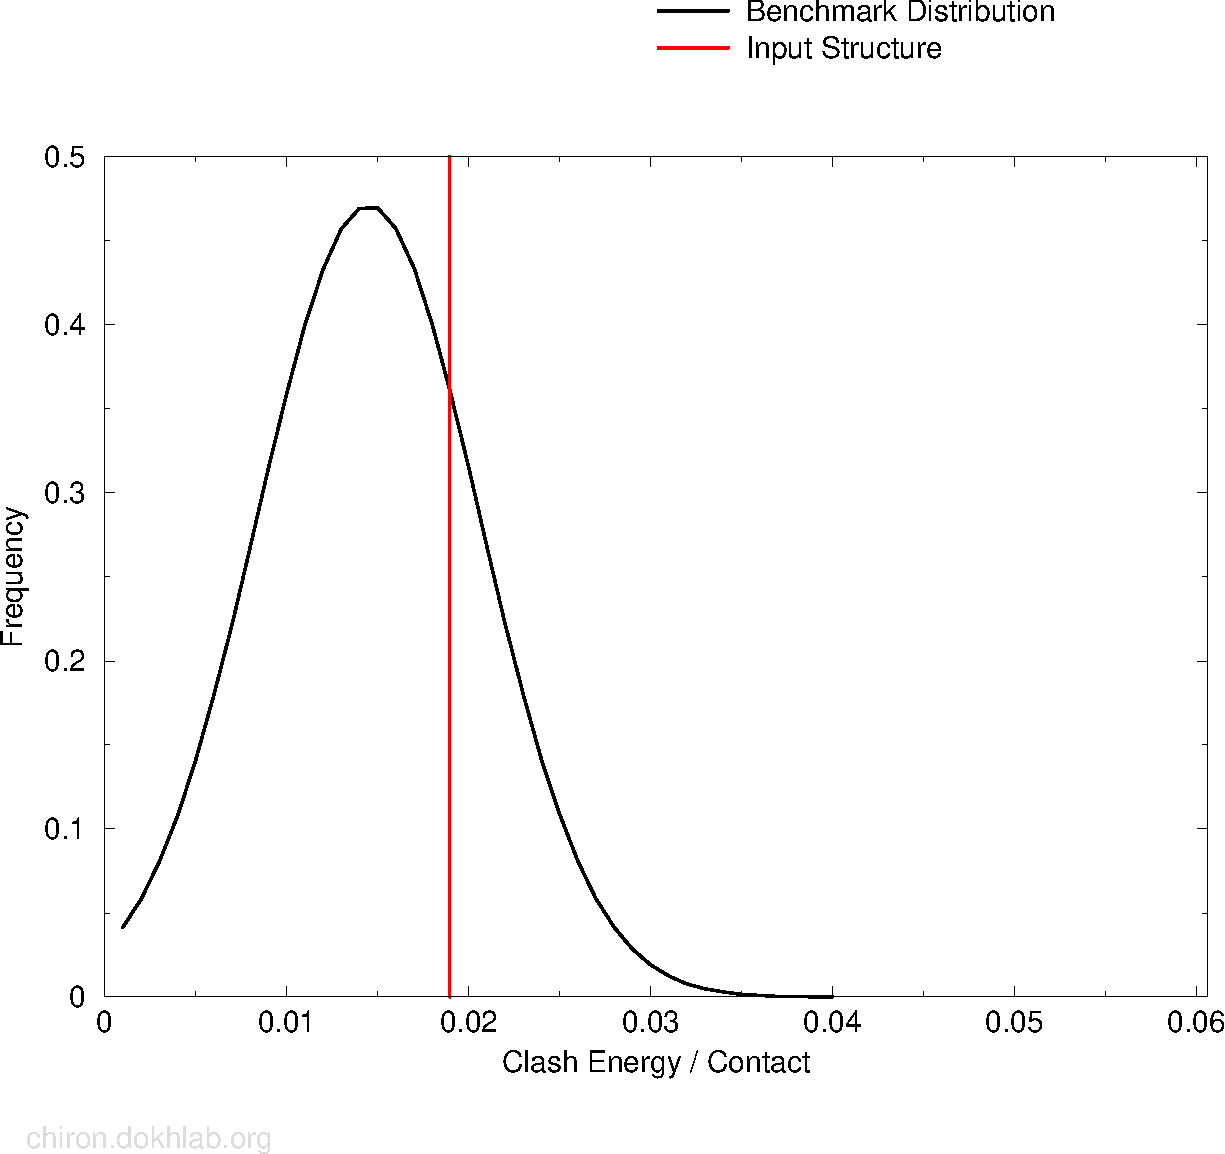
\includegraphics[width=0.75\textwidth]{4ins-678-clash.pdf}\\
		\caption{Comparison of clash-score with the distribution of clash-scores of high resolution crystal structures}
	\end{center}
\end{figure}

\begin{center}
	\begin{longtable}{lr>{\hspace{1cm}}lr>{\hspace{1cm}}r>{\hspace{1cm}}r>{\hspace{1cm}}r}
	\caption[List of clashes]{List of clashes}\\
	\toprule
	\rowcolor[gray]{0.9} \textbf{$Atom_{i}$} & \textbf{$Res_{i}$} & \textbf{$Atom_{j}$} & \textbf{$Res_{j}$} & \textbf{$d_{acc}$} & \textbf{$d_{obs}$} & \textbf{$\Delta{G}_{VDWR}$}\\
	\toprule
	\endfirsthead

	\multicolumn{7}{c}{{\bfseries \tablename\ \thetable{} -- continued from previous page}} \\
	\toprule
	\rowcolor[gray]{0.9} \textbf{$Atom_{i}$} & \textbf{$Res_{i}$} & \textbf{$Atom_{j}$} & \textbf{$Res_{j}$} & \textbf{$d_{acc}$} & \textbf{$d_{obs}$} & \textbf{$\Delta{G}_{VDWR}$}\\
	\toprule
	\endhead

	\bottomrule
	\multicolumn{7}{r}{{Continued on next page}}\\
	\bottomrule
	\endfoot
	\bottomrule
	\multicolumn{7}{r}{{End of \tablename\ \thetable{}}}\\
	\bottomrule
	\endlastfoot
		CB & 6 & SG & 11 & 3.950 & 3.029 & 0.854\\
		SG & 6 & CB & 11 & 3.950 & 2.991 & 0.915\\
		CA & 7 & SG & 28 & 4.255 & 3.260 & 0.421\\
		O & 7 & NE2 & 26 & 3.200 & 2.410 & 2.032\\
		O & 7 & CD2 & 26 & 3.598 & 3.055 & 0.503\\
		CB & 7 & SG & 28 & 3.950 & 2.953 & 0.976\\
		SG & 7 & CB & 28 & 3.950 & 3.020 & 0.868\\
		O & 9 & CD2 & 26 & 3.598 & 3.093 & 0.376\\
		CA & 11 & OE1 & 15 & 3.965 & 3.230 & 0.411\\
		CA & 20 & O & 44 & 3.965 & 3.242 & 0.387\\
		CA & 20 & SG & 40 & 4.255 & 3.281 & 0.400\\
		CB & 20 & SG & 40 & 3.950 & 3.086 & 0.765\\
		SG & 20 & CA & 40 & 4.255 & 3.309 & 0.372\\
		SG & 20 & CB & 40 & 3.950 & 2.949 & 0.981\\
		CB & 21 & O & 43 & 3.660 & 2.906 & 1.347\\
		CG & 34 & OE2 & 85 & 3.660 & 3.077 & 0.902\\
		OE2 & 34 & OE2 & 85 & 3.200 & 2.586 & 1.109\\
		O & 36 & CB & 40 & 3.660 & 3.204 & 0.372\\
		CA & 44 & O & 98 & 3.660 & 3.007 & 1.015\\
		O & 47 & CA & 95 & 3.660 & 3.174 & 0.467\\
		CA & 52 & O & 102 & 3.660 & 3.015 & 0.988\\
		O & 52 & CG & 56 & 3.660 & 3.231 & 0.301\\
		CB & 57 & SG & 62 & 3.950 & 2.886 & 1.083\\
		SG & 57 & CB & 62 & 3.950 & 3.042 & 0.833\\
		CB & 58 & SG & 79 & 3.950 & 2.997 & 0.905\\
		SG & 58 & CB & 79 & 3.950 & 3.029 & 0.855\\
		CA & 62 & OE1 & 66 & 3.965 & 3.038 & 0.809\\
		CB & 62 & OE1 & 66 & 3.660 & 3.087 & 0.753\\
		CA & 63 & ND2 & 75 & 3.965 & 3.201 & 0.576\\
		CB & 63 & ND2 & 75 & 3.660 & 3.254 & 0.301\\
		O & 65 & CB & 68 & 3.660 & 3.230 & 0.303\\
		CA & 71 & SG & 91 & 4.255 & 3.325 & 0.355\\
		CB & 71 & SG & 91 & 3.950 & 3.030 & 0.854\\
		SG & 71 & CB & 91 & 3.950 & 3.037 & 0.842\\
		O & 87 & CB & 91 & 3.660 & 3.191 & 0.413\\
	\end{longtable}
\end{center}

%List of hydrogen bonds
\clearpage
\begin{table}[!h]
	\begin{center}
		\begin{tabular}{p{16.1cm}}
			\midrule
			\cellcolor[gray]{0.9}\textbf{Hydrogen bonds}\\
			\midrule
		\end{tabular}
	\end{center}
\end{table}
\begin{center}
	\begin{longtable}{llr>{\hspace{1.2cm}}llr>{\hspace{1.2cm}}l}
	\caption[List of hydrogen bonds]{List of hydrogen bonds}\\
	\toprule
	\rowcolor[gray]{0.9} \textbf{$Atom_{i}$} & \textbf{$ResName_{i}$}  & \textbf{$Res_{i}$} & \textbf{$Atom_{j}$} & \textbf{$ResName_{j}$}  & \textbf{$Res_{j}$} & \textbf{$Type$}\\
	\toprule
	\endfirsthead

	\multicolumn{7}{c}{{\bfseries \tablename\ \thetable{} -- continued from previous page}} \\
	\toprule
	\rowcolor[gray]{0.9} \textbf{$Atom_{i}$} & \textbf{$ResName_{i}$}  & \textbf{$Res_{i}$} & \textbf{$Atom_{j}$} & \textbf{$ResName_{j}$}  & \textbf{$Res_{j}$} & \textbf{$Type$}\\
	\toprule
	\endhead

	\midrule
	\multicolumn{7}{l}{{BB - Backbone-backbone ; SS - Sidechain-sidechain ; BS/SB - Backbone-sidechain}}\\
	\bottomrule
	\multicolumn{7}{r}{{Continued on next page}}\\
	\bottomrule
	\endfoot
	\midrule
	\multicolumn{7}{l}{{BB - Backbone-backbone ; SS - Sidechain-sidechain ; BS/SB - Backbone-sidechain}}\\
	\bottomrule
	\multicolumn{7}{r}{{End of \tablename\ \thetable{}}}\\
	\bottomrule
	\endlastfoot
		N & GLY & 1 & OE1 & GLU & 4 & BS/SB\\
		N & GLU & 4 & O & GLY & 1 & BB\\
		N & GLN & 5 & O & GLY & 1 & BB\\
		NE2 & GLN & 5 & O & ILE & 10 & BS/SB\\
		N & CYS & 6 & O & ILE & 2 & BB\\
		N & CYS & 7 & O & VAL & 3 & BB\\
		N & THR & 8 & O & GLU & 4 & BB\\
		N & SER & 9 & O & GLN & 5 & BB\\
		N & CYS & 11 & O & GLN & 25 & BB\\
		N & SER & 12 & OE1 & GLN & 15 & BS/SB\\
		N & GLN & 15 & O & SER & 12 & BB\\
		N & LEU & 16 & O & SER & 12 & BB\\
		N & GLU & 17 & O & LEU & 13 & BB\\
		N & ASN & 18 & O & GLN & 15 & BB\\
		N & TYR & 19 & O & LEU & 16 & BB\\
		N & CYS & 20 & O & GLU & 17 & BB\\
		N & ASN & 21 & O & GLY & 44 & BB\\
		N & GLN & 25 & O & CYS & 11 & BB\\
		N & LEU & 27 & O & CYS & 6 & BB\\
		N & HIS & 31 & O & CYS & 28 & BB\\
		N & LEU & 32 & O & CYS & 28 & BB\\
		N & VAL & 33 & O & GLY & 29 & BB\\
		N & GLU & 34 & O & SER & 30 & BB\\
		N & ALA & 35 & O & HIS & 31 & BB\\
		N & LEU & 36 & O & LEU & 32 & BB\\
		N & TYR & 37 & O & VAL & 33 & BB\\
		N & LEU & 38 & O & GLU & 34 & BB\\
		N & VAL & 39 & O & ALA & 35 & BB\\
		N & CYS & 40 & O & LEU & 36 & BB\\
		N & GLY & 41 & O & TYR & 37 & BB\\
		N & ARG & 43 & O & CYS & 40 & BB\\
		NE & ARG & 43 & O & ASN & 21 & BS/SB\\
		NH1 & ARG & 43 & O & ASN & 21 & BS/SB\\
		N & GLY & 44 & O & CYS & 40 & BB\\
		N & PHE & 45 & O & TYR & 98 & BB\\
		N & PHE & 46 & O & TYR & 19 & BB\\
		N & TYR & 47 & O & PHE & 96 & BB\\
		N & LYS & 50 & OE2 & GLU & 4 & BS/SB\\
		N & GLY & 52 & OE2 & GLU & 55 & BS/SB\\
		N & GLU & 55 & O & GLY & 52 & BB\\
		N & GLN & 56 & O & GLY & 52 & BB\\
		NE2 & GLN & 56 & OH & TYR & 70 & SS\\
		N & CYS & 57 & O & ILE & 53 & BB\\
		N & CYS & 58 & O & VAL & 54 & BB\\
		N & THR & 59 & O & VAL & 54 & BB\\
		N & SER & 60 & O & GLU & 55 & BB\\
		N & ILE & 61 & OG & SER & 60 & BS/SB\\
		N & CYS & 62 & O & GLN & 76 & BB\\
		N & SER & 63 & OE1 & GLN & 66 & BS/SB\\
		N & GLN & 66 & O & SER & 63 & BB\\
		NE2 & GLN & 66 & OE1 & GLN & 56 & SS\\
		N & LEU & 67 & O & SER & 63 & BB\\
		N & GLU & 68 & O & LEU & 64 & BB\\
		N & ASN & 69 & O & GLN & 66 & BB\\
		N & TYR & 70 & O & LEU & 67 & BB\\
		N & CYS & 71 & O & GLU & 68 & BB\\
		N & ASN & 72 & O & GLY & 95 & BB\\
		ND2 & ASN & 72 & O & ARG & 94 & BS/SB\\
		N & GLN & 76 & O & CYS & 62 & BB\\
		ND1 & HIS & 77 & O & CYS & 58 & BS/SB\\
		N & LEU & 78 & O & CYS & 57 & BB\\
		N & HIS & 82 & O & CYS & 79 & BB\\
		N & LEU & 83 & O & CYS & 79 & BB\\
		N & VAL & 84 & O & GLY & 80 & BB\\
		N & GLU & 85 & O & SER & 81 & BB\\
		N & ALA & 86 & O & HIS & 82 & BB\\
		N & LEU & 87 & O & LEU & 83 & BB\\
		N & TYR & 88 & O & VAL & 84 & BB\\
		N & LEU & 89 & O & GLU & 85 & BB\\
		N & VAL & 90 & O & ALA & 86 & BB\\
		N & CYS & 91 & O & LEU & 87 & BB\\
		N & GLY & 92 & O & TYR & 88 & BB\\
		N & ARG & 94 & O & CYS & 91 & BB\\
		NE & ARG & 94 & O & ASN & 72 & BS/SB\\
		NH1 & ARG & 94 & O & ASN & 72 & BS/SB\\
		N & GLY & 95 & O & GLY & 92 & BB\\
		N & PHE & 96 & O & TYR & 47 & BB\\
		N & PHE & 97 & O & TYR & 70 & BB\\
		N & TYR & 98 & O & PHE & 45 & BB\\
		N & ALA & 102 & O & THR & 99 & BB\\
	\end{longtable}
\end{center}

%Unsatisfied hydrogen bonds in the shell
\newpage
\begin{table}[!h]
	\begin{center}
		\begin{tabular}{p{16.1cm}}
			\midrule
			\cellcolor[gray]{0.9}\textbf{Unsatisfied hydrogen bond partners in the shell}\\
			\midrule
		\end{tabular}
	\end{center}
\end{table}
\begin{table}[!h]
	\begin{center}
		\begin{tabular}{l@{\hspace{1cm}}c}
		\toprule
		\multicolumn{2}{c}{\cellcolor[gray]{0.9} \textbf{Shell hydrogen bond summary}} \\
			\midrule
			\# Unsatisfied partners & 40\\
			\% Unsatisfied partners & 13.80\\
			\midrule
		\end{tabular}
	\end{center}
\end{table}

\begin{figure}[h!]
	\begin{center}
		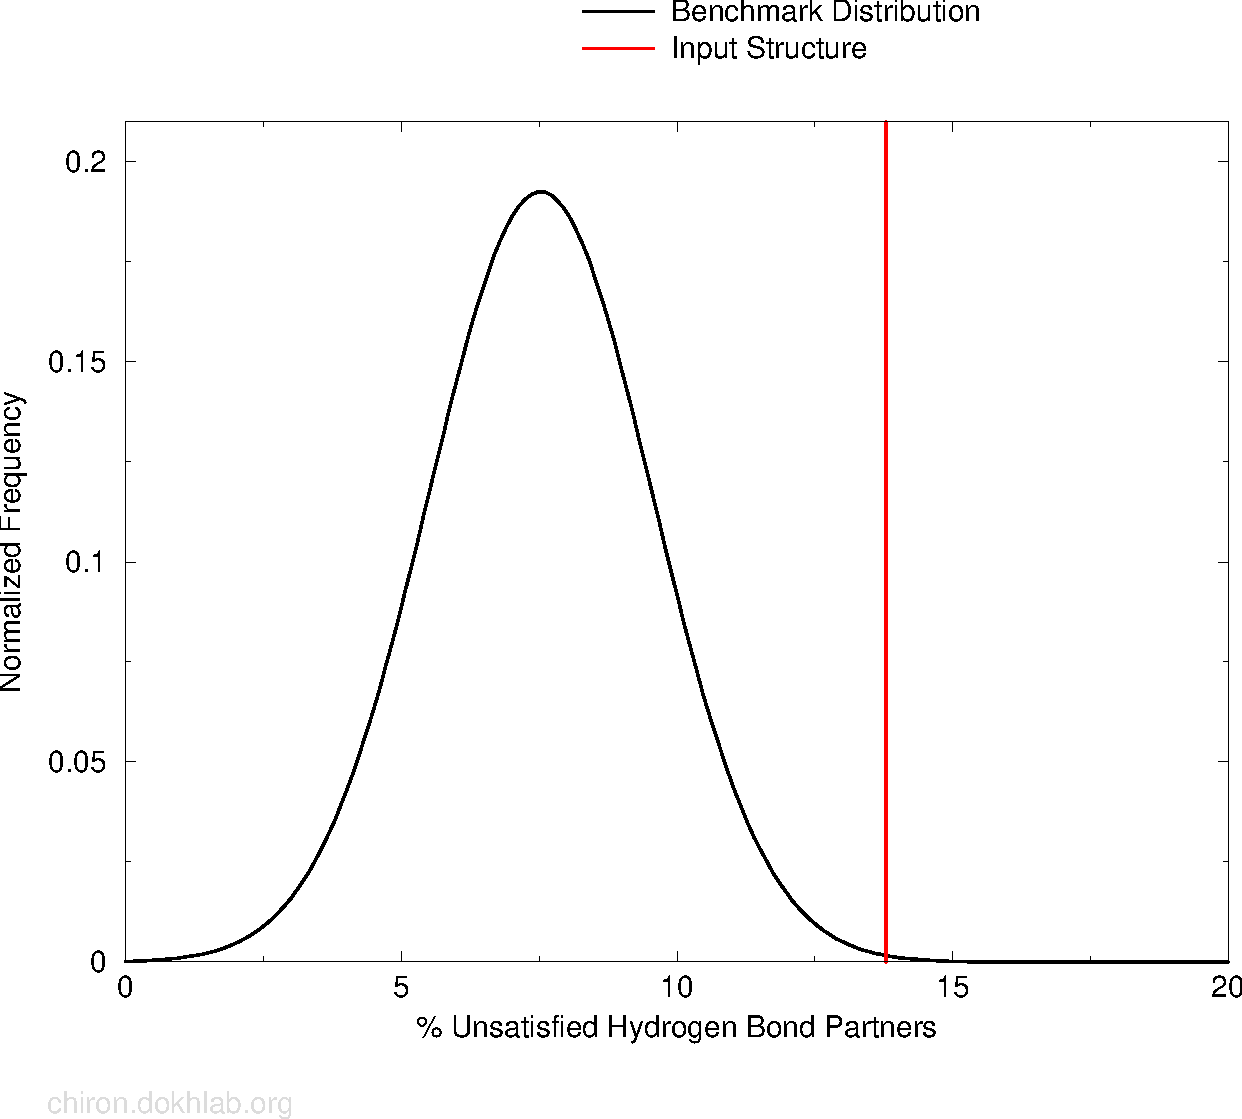
\includegraphics[width=0.75\textwidth]{4ins-678-hbond-shell.pdf}\\
		\caption{Comparison of \%unsatisfied hydrogen bonds in the shell with the distribution from high resolution crystal structures}
	\end{center}
\end{figure}

%List of unsatisfied partners in the shell
\clearpage
\begin{center}
	\begin{longtable}{l>{\hspace{1.2cm}}l>{\hspace{1.2cm}}r}
	\caption[List of unsatisfied partners in the shell]{List of unsatisfied partners in the shell}\\
	\toprule
	\rowcolor[gray]{0.9} \textbf{$Atom$} & \textbf{$ResName$}  & \textbf{$Res$}\\
	\toprule
	\endfirsthead

	\multicolumn{3}{c}{{\bfseries \tablename\ \thetable{} -- continued from previous page}} \\
	\toprule
	\rowcolor[gray]{0.9} \textbf{$Atom$} & \textbf{$ResName$}  & \textbf{$Res$}\\
	\toprule
	\endhead

	\bottomrule
	\multicolumn{3}{r}{{Continued on next page}}\\
	\bottomrule
	\endfoot
	\bottomrule
	\multicolumn{3}{r}{{End of \tablename\ \thetable{}}}\\
	\bottomrule
	\endlastfoot
		N & ILE & 2\\
		N & VAL & 3\\
		N & ILE & 10\\
		SG & CYS & 11\\
		N & LEU & 13\\
		N & TYR & 14\\
		SG & CYS & 20\\
		ND2 & ASN & 21\\
		N & VAL & 23\\
		O & VAL & 23\\
		N & ASN & 24\\
		N & HIS & 26\\
		NE2 & HIS & 26\\
		O & LEU & 27\\
		N & CYS & 28\\
		SG & CYS & 40\\
		O & GLY & 41\\
		N & GLU & 42\\
		O & GLU & 42\\
		O & PHE & 46\\
		N & THR & 48\\
		N & ALA & 51\\
		N & VAL & 54\\
		O & GLN & 56\\
		O & SER & 60\\
		N & LEU & 64\\
		N & TYR & 65\\
		SG & CYS & 71\\
		N & VAL & 74\\
		O & VAL & 74\\
		N & ASN & 75\\
		N & HIS & 77\\
		O & LEU & 78\\
		N & CYS & 79\\
		SG & CYS & 91\\
		N & GLU & 93\\
		O & PHE & 97\\
		N & THR & 99\\
		N & LYS & 101\\
		O & ALA & 102\\
	\end{longtable}
\end{center}

%Unsatisfied hydrogen bonds in the core
\newpage
\begin{table}[!h]
	\begin{center}
		\begin{tabular}{p{16.1cm}}
			\midrule
			\cellcolor[gray]{0.9}\textbf{Unsatisfied hydrogen bond partners in the core}\\
			\midrule
		\end{tabular}
	\end{center}
\end{table}
\begin{table}[!h]
	\begin{center}
		\begin{tabular}{l@{\hspace{1cm}}c}
		\toprule
		\multicolumn{2}{c}{\cellcolor[gray]{0.9} \textbf{Core hydrogen bond summary}} \\
			\midrule
			\# Unsatisfied partners & 4\\
			\% Unsatisfied partners & 1.30\\
			\midrule
		\end{tabular}
	\end{center}
\end{table}

\begin{figure}[h!]
	\begin{center}
		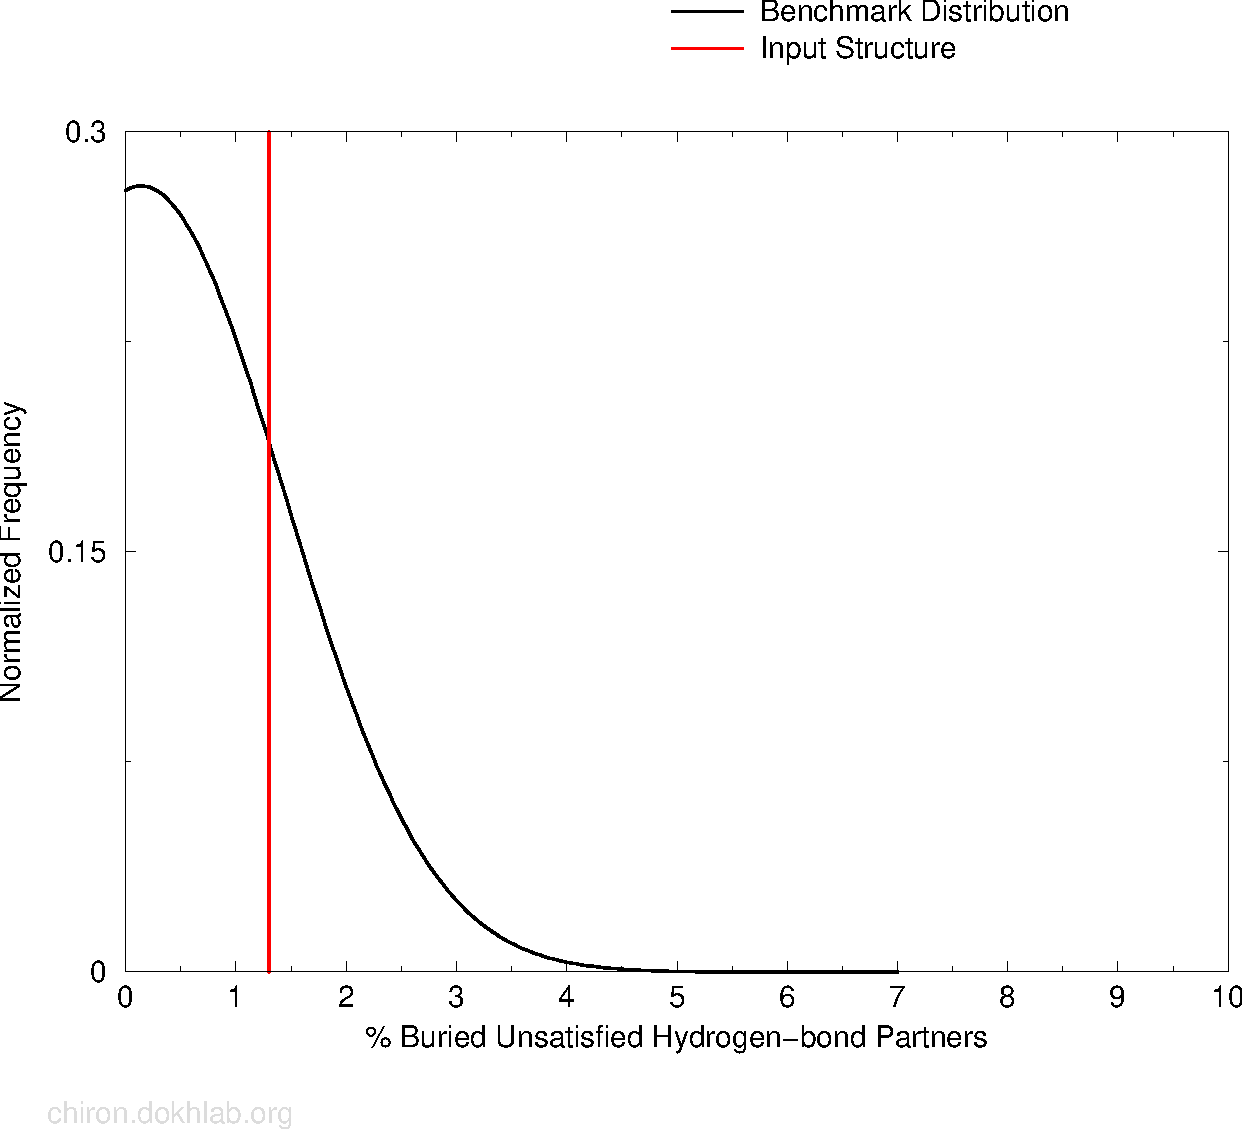
\includegraphics[width=0.75\textwidth]{4ins-678-hbond-buried.pdf}\\
		\caption{Comparison of \%unsatisfied hydrogen bonds in the core with the distribution from high resolution crystal structures}
	\end{center}
\end{figure}

%List of unsatisfied partners in the core
\clearpage
\begin{center}
	\begin{longtable}{l>{\hspace{1.2cm}}l>{\hspace{1.2cm}}r}
	\caption[List of unsatisfied partners in the core]{List of unsatisfied partners in the core}\\
	\toprule
	\rowcolor[gray]{0.9} \textbf{$Atom$} & \textbf{$ResName$}  & \textbf{$Res$}\\
	\toprule
	\endfirsthead

	\multicolumn{3}{c}{{\bfseries \tablename\ \thetable{} -- continued from previous page}} \\
	\toprule
	\rowcolor[gray]{0.9} \textbf{$Atom$} & \textbf{$ResName$}  & \textbf{$Res$}\\
	\toprule
	\endhead

	\bottomrule
	\multicolumn{3}{r}{{Continued on next page}}\\
	\bottomrule
	\endfoot
	\bottomrule
	\multicolumn{3}{r}{{End of \tablename\ \thetable{}}}\\
	\bottomrule
	\endlastfoot
		SG & CYS & 6\\
		N & ILE & 53\\
		SG & CYS & 57\\
		SG & CYS & 62\\
	\end{longtable}
\end{center}

%Solvent excluded surface area
\newpage
\begin{table}[!h]
	\begin{center}
		\begin{tabular}{p{16.1cm}}
			\midrule
			\cellcolor[gray]{0.9}\textbf{Solvent excluded surface area (SASA)}\\
			\midrule
		\end{tabular}
	\end{center}
\end{table}

\begin{table}[!h]
	\begin{center}
		\begin{tabular}{l@{\hspace{1cm}}c}
		\toprule
		\multicolumn{2}{c}{\cellcolor[gray]{0.9} \textbf{MSA summary}} \\
			\midrule
			Total MSA & 4869.93\\
			Rescaled MSA & 119.47\\
			\midrule
		\end{tabular}
	\end{center}
\end{table}

\begin{figure}[h!]
	\begin{center}
		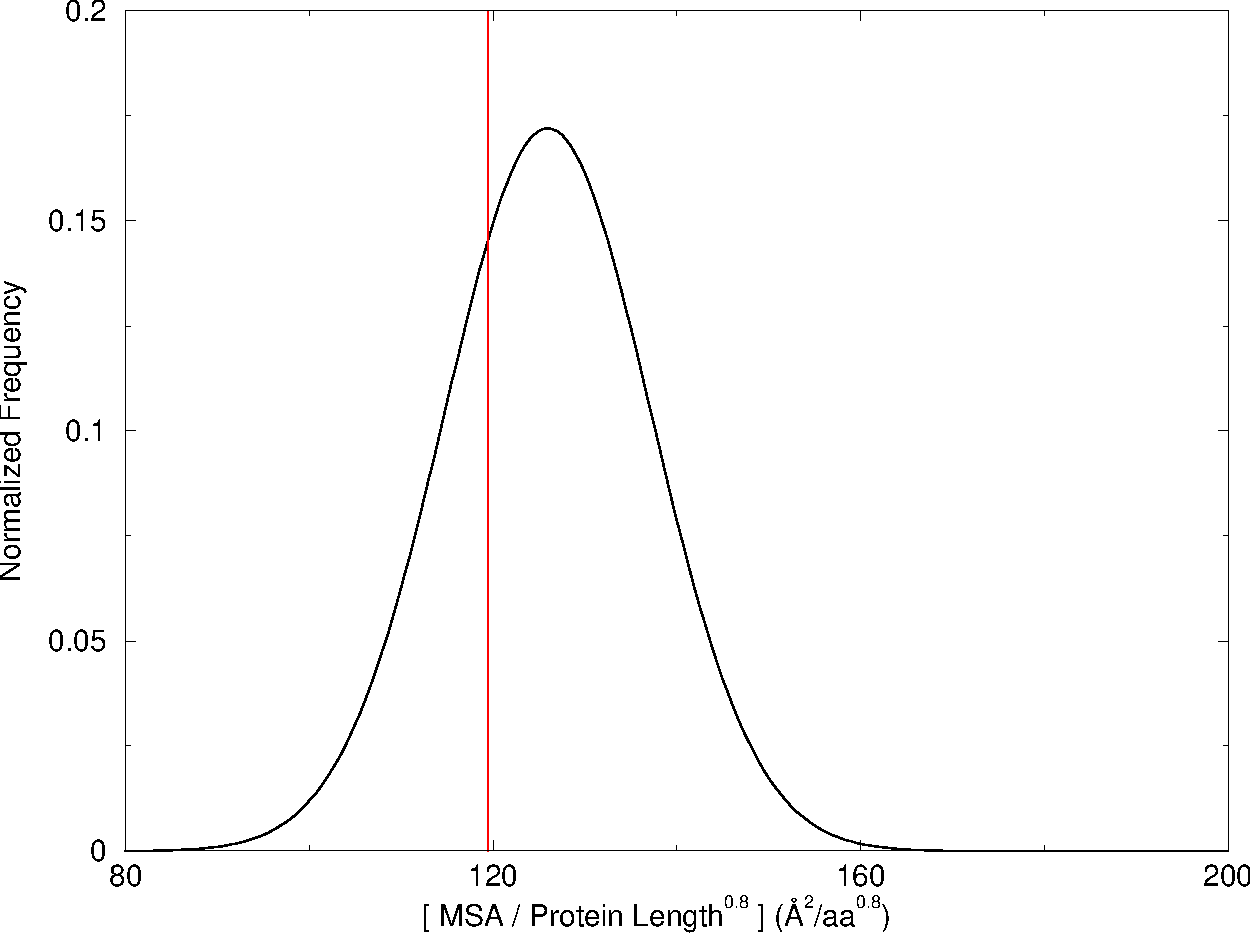
\includegraphics[width=0.75\textwidth]{4ins-678-msa.pdf}\\
		\caption{Comparison of rescaled solvent excluded surface area with the distribution from high resolution crystal structures}
	\end{center}
\end{figure}

%Void volume
\newpage
\begin{table}[!h]
	\begin{center}
		\begin{tabular}{p{16.1cm}}
			\midrule
			\cellcolor[gray]{0.9}\textbf{Void volume}\\
			\midrule
		\end{tabular}
	\end{center}
\end{table}

The total void volume of the input structure is \textbf{51.08} ${\mathring{A}\textsuperscript{3}}$. In order to eliminate bias due to length of the protein, we normalize the void volume by the chain length. The rescaled volume of the input structure is \textbf{0.50} ${\mathring{A}\textsuperscript{3}}$. The red line in the plot above represents the rescaled void volume of the input structure in context of the distribution generated from high resolution crystal structures.

\begin{figure}[h!]
	\begin{center}
		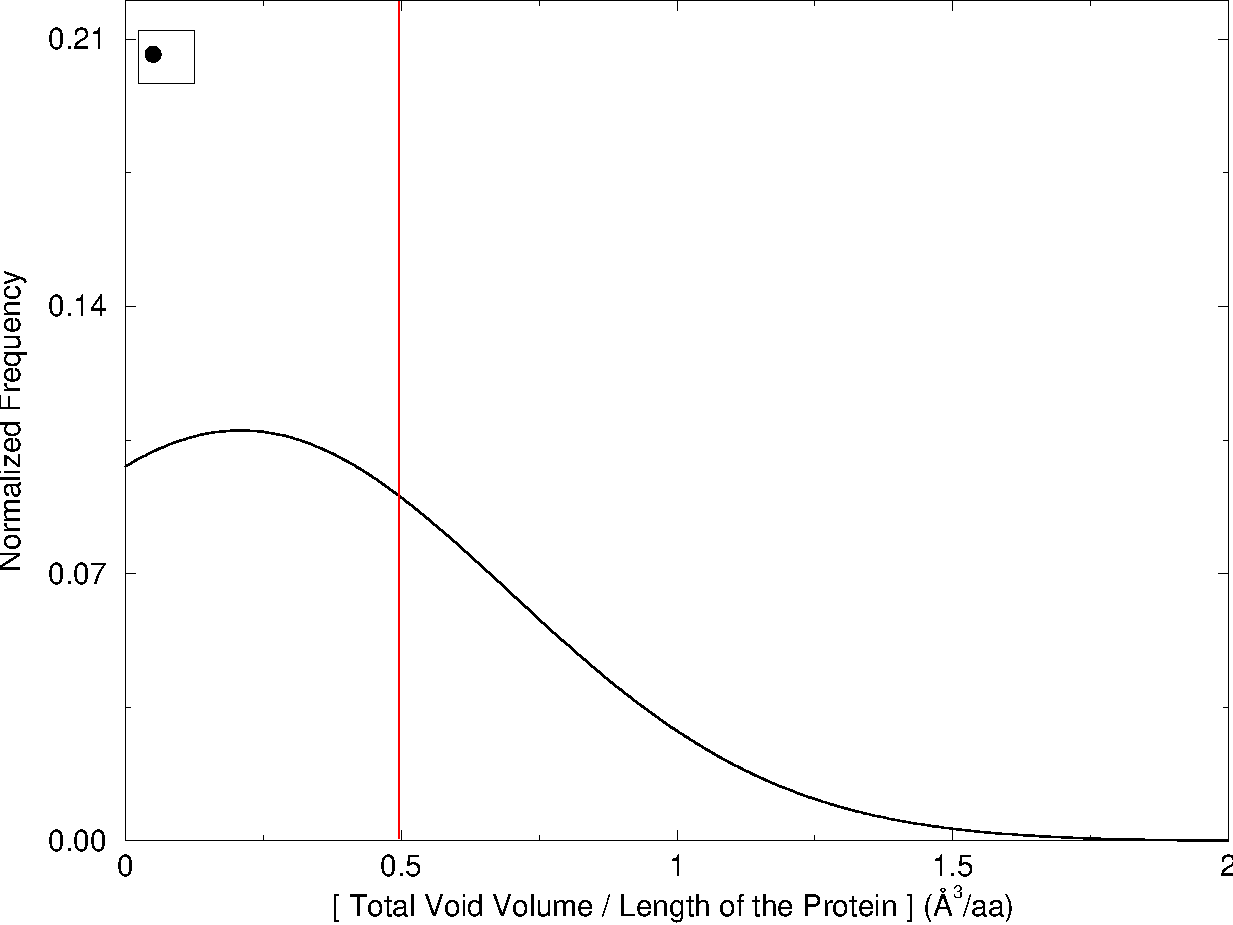
\includegraphics[width=0.75\textwidth]{4ins-678-voids.pdf}\\
		\caption{Comparison of rescaled void volume with the distribution from high resolution crystal structures}
	\end{center}
\end{figure}

%List of voids
\clearpage
\begin{center}
	\begin{longtable}{r>{\hspace{1.2cm}}r}
	\caption[List of voids]{List of voids}\\
	\toprule
	\rowcolor[gray]{0.9} \textbf{$Void$} & \textbf{$Volume (\mathring{A}\textsuperscript{3})$}\\
	\toprule
	\endfirsthead

	\multicolumn{2}{c}{{\bfseries \tablename\ \thetable{} -- continued from previous page}} \\
	\toprule
	\rowcolor[gray]{0.9} \textbf{$Void$} & \textbf{$Volume (\mathring{A}\textsuperscript{3})$}\\
	\toprule
	\endhead

	\bottomrule
	\multicolumn{2}{r}{{Continued on next page}}\\
	\bottomrule
	\endfoot
	\bottomrule
	\multicolumn{2}{r}{{End of \tablename\ \thetable{}}}\\
	\bottomrule
	\endlastfoot
		1 & 0.000\\
		2 & 0.000\\
	\end{longtable}
\end{center}

\end{document}
%----End Document----%
